\chapter{Výsledky a Záver}

\section{Testovanie}
Pri testovaní vizualizácie sme postupovali podľa článku od Elmqvist et al. \cite{Patterns}, ktorý opisuje najpoužívanejšie vzory testovania vizualizácie a článok od Vogel et al., v ktorom autori testujú webovú vizualizáciu \cite{WebBasedUserTest}.

\subsection{Testovacia procedúra}
Testovanie prebiehalo prostredníctvom niekoľkých úloh, ktoré sme navrhli na základe špecifikácie požiadaviek na vizualizáciu uvedených v sekcii \ref{sec:spec}. 

Každému subjektu bola predstavená základná funkcionalita systému v krátkom 15 minútovom návode. Následne subjekt obdržal testovací formulár (pozri prílohu \ref{sec:testform}) obsahujúci 7 rôznych úloh, ktoré mal subjekt vykonať a po vykonaní každej z nich do formulára zapísať výsledok svojho skúmania.

Pri testovaní sme jednak vyhodnocovali správnosť odpovedí ale aj rýchlosť vykonania jednotlivých úloh. Taktiež sme dokumentovali interakciu s vizualizáciou počas vykonávania úlohy pomocou \textit{screen capture}.

\subsection{Výsledky testovania}

Vizualizáciu sme testovali na 6 subjektoch bez vyššieho meteorologického, matematického alebo informatického vzdelania. Taktiež žiaden užívateľ nemal skúsenosti s verifikáciou predpovedí a náš systém videl prvýkrát v živote. Všetky tieto faktory vplývali na výsledok nášho testu, keďže sme sa často stretali s nepochopením respektíve s pomalým pochopením zadania a teda čas riešenia úlohy sa značne natiahol.

V tabuľke \ref{table:results} môžme vidieť, že všetci testovaní užívatelia vyriešili všetky úlohy správne a výsledky riešenia sa líšili iba v nameranom čase. V tabuľke je hrubým písmom zvýraznený najdlhší a najkratší priemerný čas pre dané úlohy. 
V priemere každá úloha trvala asi pol minúty (26s) a všetky úlohy užívatelia vykonali v priemere za 3 minúty.


\begin{table}[h]
\centering
\caption{Výsledky testovania}
\label{table:results}
\begin{tabular}{|c|c|c|c|}
\hline
\rowcolor[HTML]{9B9B9B} \textbf{Úloha} & \textbf{Počet správnych} & \textbf{Počet nesprávnych} & \textbf{Priemerný čas} \\ \hline
1              &            6             &             0              &         23.85s                       \\ \hline
2              &            6             &             0              &         37.27s                      \\ \hline
3              &            6             &             0              &         24.66s                      \\ \hline
4              &            6             &             0              &         \textbf{40.36}s                      \\ \hline
5              &            6             &             0              &         24.69s                      \\ \hline
6              &            6             &             0              &         \textbf{9.73}s                      \\ \hline
7              &            6             &             0              &         23.27s                       \\ \hline
\rowcolor[HTML]{C0C0C0} \textbf{Suma}  &           \textbf{42}             &             \textbf{0}              &        \textbf{183.83}                      \\ \hline
\end{tabular}
\end{table}

V grafe na obrázku \ref{fig:results} môžme lepšie vidieť sumárne porovnanie časov pre jednotlivé úlohy a užívateľov. Môžme si ľahko všimnúť, že úlohy 1, 2, 5 a 7 majú približne rovnaký priemerný čas, zatiaľ čo úlohy 2, 4 mali výrazne dlhšie trvanie a úloha 9 trvala v priemere najkratšie.

Dlhé trvanie úlohy 2 prisudzujeme vyššej zložitosti úlohy oproti ostatným. Pre užívateľov bolo odhalenie outlierov pomerne rýchle, avšak väčšinu času zabralo užívateľom odčítanie z grafu o akú presnú hodnotu a predpoveď ide.

Pri úlohe 4 bolo problémom rýchle odčítanie z grafu, o aký dátum sa jedná. Dôvodom bolo nedobré označenie dátumov na \mbox{$ x $-ovej} škále, kedy sa jednotlivé dni v roku označujú číslami 0-364. Užívateľ uvidel konkrétny dátum, až keď nadišiel myšou na dané miesto, kedy sa mu presné hodnoty ukázali v \textit{tooltipe}. Lepším riešením by bola redšia škála s mesačnými intervalmi alebo konkrétnymi dátumami.

Výsledky nášho testovania považujeme celkovo za uspokojivé, keďže aj neskúsení užívatelia dosahovali pri všetkých úlohách dobré časy. Taktiež nám tieto výsledky poukázali na slabiny našej práce, ktorými sú hlavne zlé alebo slabé označenia škál, grafov a legiend.

\begin{figure}
	\centering
	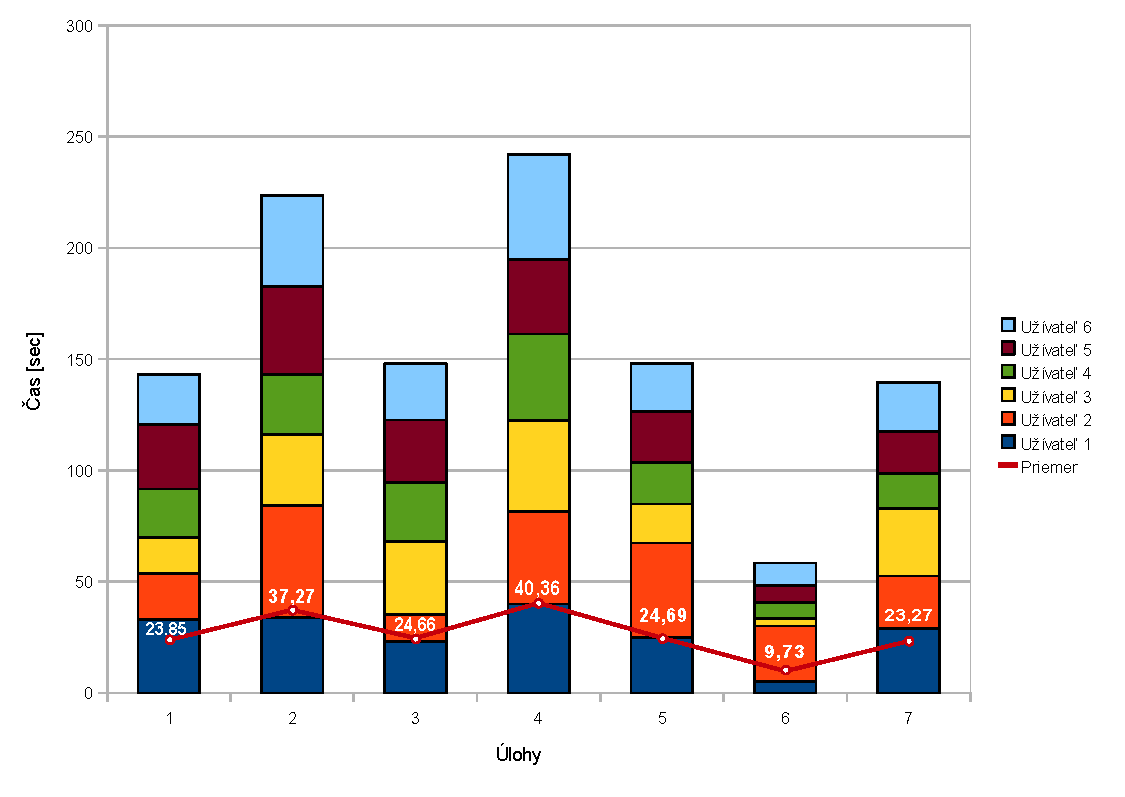
\includegraphics[width = 5in]{resultchart}
	\caption{Výsledky testovania.}
	\label{fig:results} 
\end{figure}

%TODO \section{Demonštrácia}

\section{Záver}
V našej práci sme uviedli problém verifikácie predpovedných modelov počasia so zameraním na verifikáciu predpovede spojitej premennej v jednom bode. Zhrnuli sme používané štatistické metódy na meranie chyby predpovede a navrhli sme spôsob všeobecného výpočtu kumulovanej chyby, ktorý sme v závere využili aj pri implementácii.

Taktiež sme preskúmali doterajšie riešenia jednak z pohľadu verifikačného softvéru, ale aj z pohľadu vizualizačných techník vo verifikácii. Uviedli sme slabé a silné stránky jednotlivých softvérových riešení a zhrnuli sme ich v prehľadnej tabuľke. Taktiež sme opísali a analyzovali vizualizácie používané vo verifikácii a načrtli ich zameranie a spôsob použitia.

Ďalej sme charakterizovali vstupné dáta a špecifikovali požiadavky používateľov, na základe ktorých sme navrhli rôzne spôsoby vizualizácie, ktoré sme implementovali ako doplnok JavaScriptovej knižnice D3. V závere práce sme následne vykonali testovanie našej vizualizácie na základe čoho sme zhodnotili jej úspešnosť.

Výsledkom práce je teda verifikačný nástroj schopný spracovávať dáta z rôznych zdrojov, ponúkajúc funkcionalitu pre verifikáciu predpovedí spojitej premennej s použitím špeciálne navrhnutej vizualizácie pre tieto účely. 

\subsubsection{Prínos}

Za hlavný prínos tejto práce považujeme práve návrh špecializovanej vizualizácie, ktorá síce nevyniká obrovskou inováciou, ale pri jej vzniku sme navrhli mnoho drobných originálnych vylepšení smerujúcim k lepšiemu, rýchlejšiemu a jednoduchšiemu porozumeniu dát. Príkladom môže byť návrh prehľadovej vizualizácie verifikačných dát, návrh riešenia viacerých škál pri \mbox{mnoho-čiarovom} diagrame, zovšeobecnenie re-dizajnu krabicového diagramu od \mbox{Bada et. al.} \cite{Bade} na takzvaný \textit{Pruhový diagram}, využitie dvojtónového pseudofarbenia pri kompaktnej vizualizácii distribúcie dát pomocou grafu hustoty a podobne.

\subsubsection{Budúca práca}

Na výskum a vývoj neustále existuje priestor a v našej práci ho vidíme určite mnoho obzvlášť v štyroch oblastiach:
\begin{enumerate}
	\item \textit{Získavanie dát} - V práci sme implementovali 3 typy zdrojov: Grib, CSV a Web. Avšak existuje mnoho ďalších zdrojov dát, z kade možno získať pozorovania, rovnako ako aj predpovede. Príkladom je napríklad \textit{databáza}, \textit{XML}, alebo \textit{XLS} súbory, takzvané \textit{bloky} systému IMS4, kde sú aj merania a mnohé iné ďalšie zdroje. 
	\item \textit{Konfigurácia systému a vizualizácie} - Konfigurovanie systému v momentálnom stave nie je veľmi user-friendly úloha. V budúcej práci očakávame návrh riešenia, ktoré skryje pred užívateľom pomerne neprehľadné nastavenia systému.
	\item \textit{Interaktívna manipulácia s dátami} - Momentálne riešenie neponúka veľmi dôležitú súčasť moderných vizualizačných nástrojov a tým je manipulácia s dátami priamo na obrazovke. Príkladmi operácií môže byť filtrovanie dát na základe rôznych kľúčov alebo selekcia vybranej vzorky dát pomocou \textit{brushingu} a podobne.
	\item \textit{Porovnávanie modelov a staníc} - Pri návrhu vizualizácie sme nezvažovali možnosť porovnávania výkonu viacerých predpovedných modelov alebo porovnávanie predpovedí pre rôzne stanice súčasne. Riešenie takéhoto problému by pravdepodobne vyžadovalo zásadný re-dizajn vizualizácie.
\end{enumerate}